\section{Experiments and Results}
\label{sec:experiments}

\subsection{Experimental Setup}

\textbf{Evaluation Protocol.} We use 5-fold stratified cross-validation on the merged training+validation set (2,266 samples) to generate out-of-fold (OOF) predictions. All folds use \texttt{random\_state=42} for reproducibility. The primary metric is Micro-F1 (equals accuracy for multi-class), matching the Kaggle competition metric.

\textbf{Baselines.} A majority-class classifier achieves 46.6\% Micro-F1. Random with class-proportional sampling achieves $\sum_c p_c^2 \approx 36.9\%$.

\textbf{Dataset splits:} Train=1,983, Val=283, Test=378 (new\_test).

\subsection{Modality Solo Performance}

Before building combined models, we measured the standalone discriminative power of each data source using 5-fold CV (ML\_experiments.ipynb Cell 6). This ranking directly motivated our architecture design. Figure~\ref{fig:solo_modality} (Section~\ref{sec:modalities}) shows the solo performance of each modality.

\begin{table}[H]
\centering
\caption{Solo modality Micro-F1 (5-fold CV). Data from ML\_experiments.ipynb Cell 6.}
\label{tab:solo_modality}
\begin{tabular}{llrc}
\toprule
\textbf{Modality} & \textbf{Best Model} & \textbf{Dim} & \textbf{Micro-F1} \\
\midrule
Report (TF-IDF+SVD-64) & SVM-RBF & 64 & 84.29\% \\
Clinical + SI & RF & 27 & 66.51\% \\
Location (label-enc) & LGB ensemble & 1 & 62.67\% \\
Image (PCA pooled) & RF & 128 & 56.97\% \\
Radiomics (raw) & RF & 20 & 52.21\% \\
\midrule
\multicolumn{3}{l}{Majority-class baseline} & 46.6\% \\
\bottomrule
\end{tabular}
\end{table}

Three key observations: (1) Reports dominate at 84.29\%, surpassing all other modalities combined. (2) Radiomics barely exceed the majority baseline (52.21\% vs 46.6\%). (3) The gap between reports and other modalities ($>$18\%) means the architecture must prioritize the report path.

\subsection{Class Imbalance Handling}

The dataset exhibits a 40:1 imbalance ratio (Glioma 46.6\% vs Pineal/CP 1.1\%). Since Micro-F1 equals accuracy in multi-class and is dominated by majority classes (Glioma + Meningioma = 83.3\% of data), there is a tension between optimizing Micro-F1 and maintaining minority-class performance.

To determine the right strategy, we swept class weight strength $\alpha \in \{0, 0.25, 0.5, 0.75, 1.0\}$ on XGBoost (TF-IDF + tabular features), where $\alpha=0$ means no weights and $\alpha=1.0$ means full balanced weights.

\begin{table}[H]
\centering
\caption{Class weight sweep (XGBoost, 5-fold CV). Adding weights to tree models hurts Micro-F1. Data from model\_final.ipynb Cell 28.}
\label{tab:weight_sweep}
\begin{tabular}{lccc}
\toprule
\textbf{Strategy} & \textbf{Micro-F1} & \textbf{Macro-F1} & \textbf{Pineal/CP Acc} \\
\midrule
No weights ($\alpha$=0) & 85.04\% & 68.99\% & 15.33\% \\
Mild ($\alpha$=0.25) & 84.82\% & \textbf{70.61\%} & 23.33\% \\
Sqrt ($\alpha$=0.5) & 83.89\% & 69.53\% & 23.33\% \\
Strong ($\alpha$=0.75) & 82.04\% & 68.30\% & 26.67\% \\
Balanced ($\alpha$=1.0) & 79.44\% & 66.11\% & 30.00\% \\
\bottomrule
\end{tabular}
\end{table}

\begin{figure}[H]
\centering
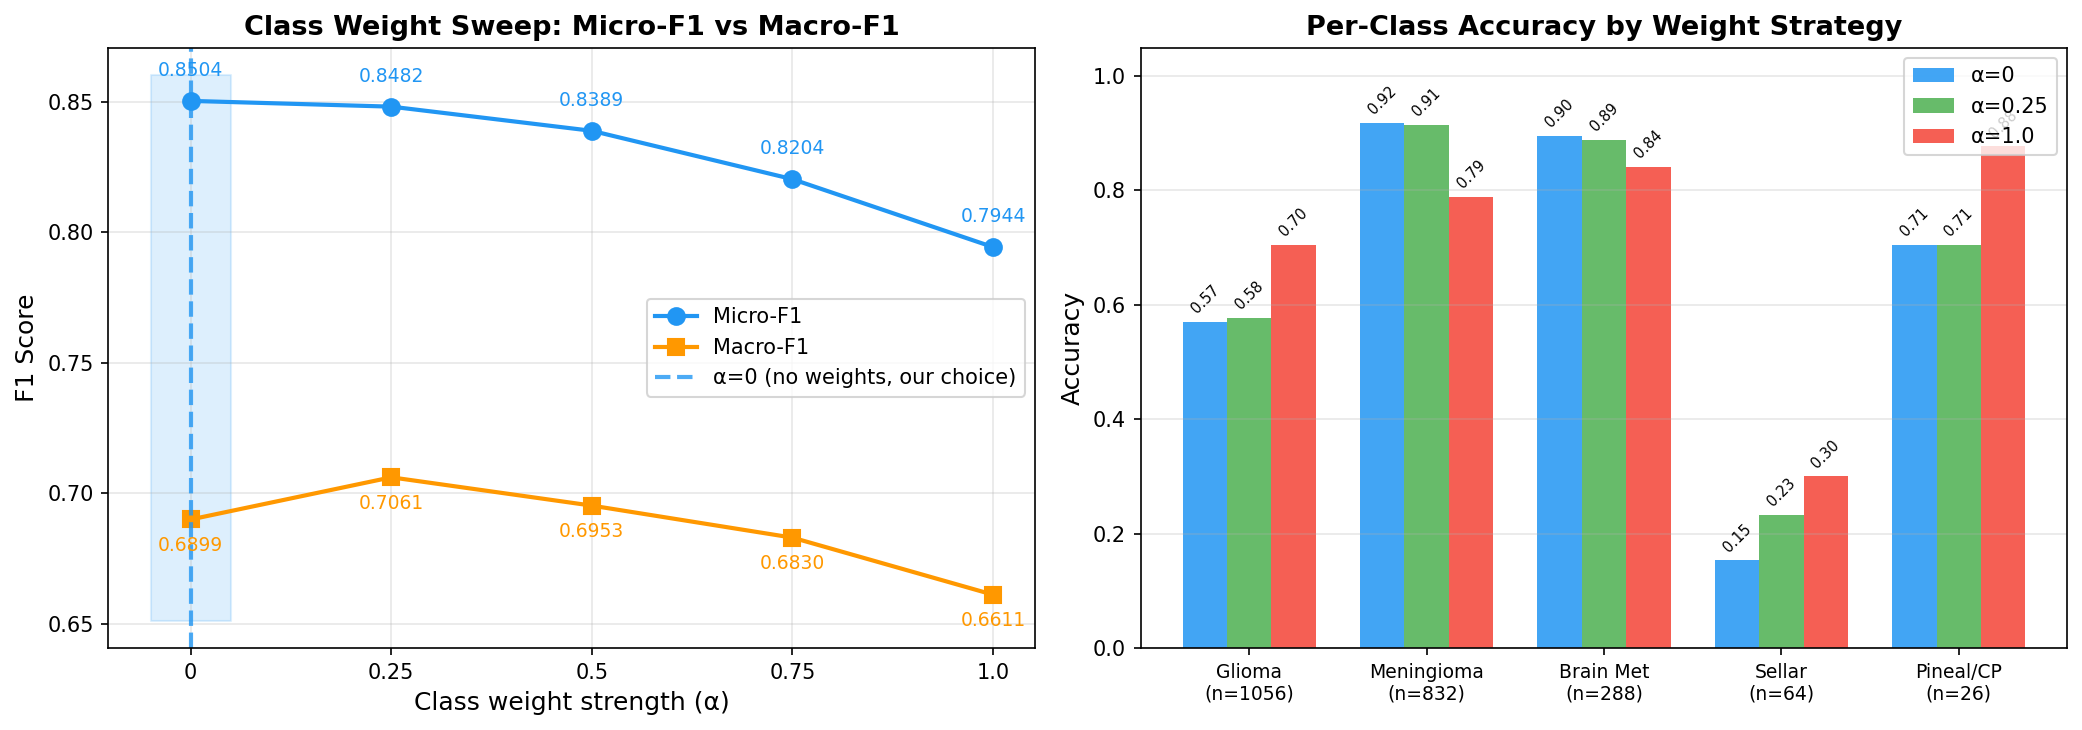
\includegraphics[width=0.9\textwidth]{figures/class_weight_sweep.png}
\caption{Class weight sweep: Micro-F1 vs Macro-F1 by α (left) and per-class accuracy by weight strategy (right).}
\label{fig:class_weight_sweep}
\end{figure}

The results show a clear trade-off: increasing $\alpha$ improves minority-class recall (Pineal/CP: 15.3\% $\to$ 30.0\%) but at severe cost to Micro-F1 (85.04\% $\to$ 79.44\%). Even mild weighting ($\alpha=0.25$) drops Micro-F1 by 0.22\% with negligible Macro-F1 gain. Since gradient-boosted trees already handle imbalance through sequential error correction, explicit class weights are redundant and harmful.

\textbf{Our strategy:} Tree models use no class weights ($\alpha=0$). The neural network uses \emph{sqrt class weights} ($\alpha=0.5$), which is appropriate because NNs lack the built-in error-correction mechanism of boosting and benefit from a gentle minority boost. Label smoothing (0.05) in the NN also serves as an implicit regularizer against overconfidence on majority classes.

\subsection{Neural Network Training}

We train the dual-path neural network (Section~\ref{sec:nn}) with 5-fold OOF evaluation. Each fold trains on $\sim$1,813 samples.

\textbf{Training configuration:} Main LR=$3\times10^{-5}$, BERT LR scale=0.05, Label smoothing=0.05, Sqrt class weights ($\alpha=0.5$), Cosine annealing + 3-epoch warmup, SWA from 70\% of epochs, Early stopping (patience=25).

\textbf{NN 5-Fold OOF Micro-F1: 82.35\%.} Per-fold OOF scores show variation across folds reflecting differences in class composition, particularly for minority classes with as few as 5 Pineal/CP samples per fold.

\subsection{Tree Model Results}

We train three categories of tree models with 5-fold OOF (model\_final.ipynb Cell 20):

\begin{itemize}
  \item \textbf{MLU Models:} XGBoost, LightGBM, CatBoost on Report SVD-256 + Clinical+SI (27d) + Location hierarchy (3d) + Cross-modal Ratios (25d) + SI unknown (1d) = 312d
  \item \textbf{NNXGB:} XGBoost on NN OOF probabilities (5d). The NN acts as a learned encoder that compresses reports and tabular data into a 5-class probability vector; XGBoost then corrects the NN's systematic errors on this representation.
  \item \textbf{ImgTab:} XGBoost on Image PCA (512d) + Tabular ($\sim$57d) = 569d
\end{itemize}

\begin{table}[H]
\centering
\caption{Tree model OOF performance (5-fold CV). Data from model\_final.ipynb Cell 20.}
\label{tab:tree_models}
\begin{tabular}{llcc}
\toprule
\textbf{Model} & \textbf{Features} & \textbf{Micro-F1} & \textbf{Macro-F1} \\
\midrule
MLU-XGB (XGBoost) & Report SVD-256 + Tabular (312d) & \textbf{86.28\%} & \textbf{73.16\%} \\
MLU-LGB (LightGBM) & Report SVD-256 + Tabular (312d) & 85.97\% & 71.80\% \\
MLU-CB (CatBoost) & Report SVD-256 + Tabular (312d) & 85.70\% & 72.64\% \\
NNXGB (XGBoost) & NN OOF probs (5d) & 77.27\% & 67.60\% \\
ImgTab (XGBoost) & Image PCA + Tabular (569d) & 69.77\% & 47.45\% \\
\midrule
NN (Neural Network) & BERT + Tabular & 82.35\% & 71.15\% \\
\bottomrule
\end{tabular}
\end{table}

% FIGURE: model_comparison.png — GENERATE
%
% Lollipop chart (dot + stem) showing individual model OOF Micro-F1.
% Vertical stems with dots at top, sorted by F1 ascending (bottom to top).
% Each model is a row. Dot size proportional to its ensemble weight.
% Color groups: Green (MLU tree models), Blue (NN), Purple/Orange (auxiliary).
% A vertical dashed reference line at 46.6% (baseline).
% A shaded band from 85.70%–86.28% labeled "MLU range (0.58% spread)".
%
% Data (from model_final.ipynb Cell 20):
%   ImgTab  = 69.77%  dot_size=0%,             orange
%   NNXGB   = 77.27%  dot_size=0%,              purple
%   NN      = 82.35%  dot_size=40% (largest),  blue
%   MLU-LGB = 85.97%  dot_size=30%,            green
%   MLU-XGB = 86.28%  dot_size=30%,             green
%   MLU-CB  = 85.70%  dot_size=0% (excluded),  green
%
% Annotation: Arrow from NN dot saying "40% weight"
%             Bracket over MLU models saying "2 of 3 algorithms weighted"
%             Small text on ImgTab: "Different signal (image)"
%
% Title: "Model Performance & Ensemble Role (5-Fold OOF)"
% X-axis: "Micro-F1 (%)"   Y-axis: model names
% Figure size: (10, 5)
%
\begin{figure}[H]
\centering
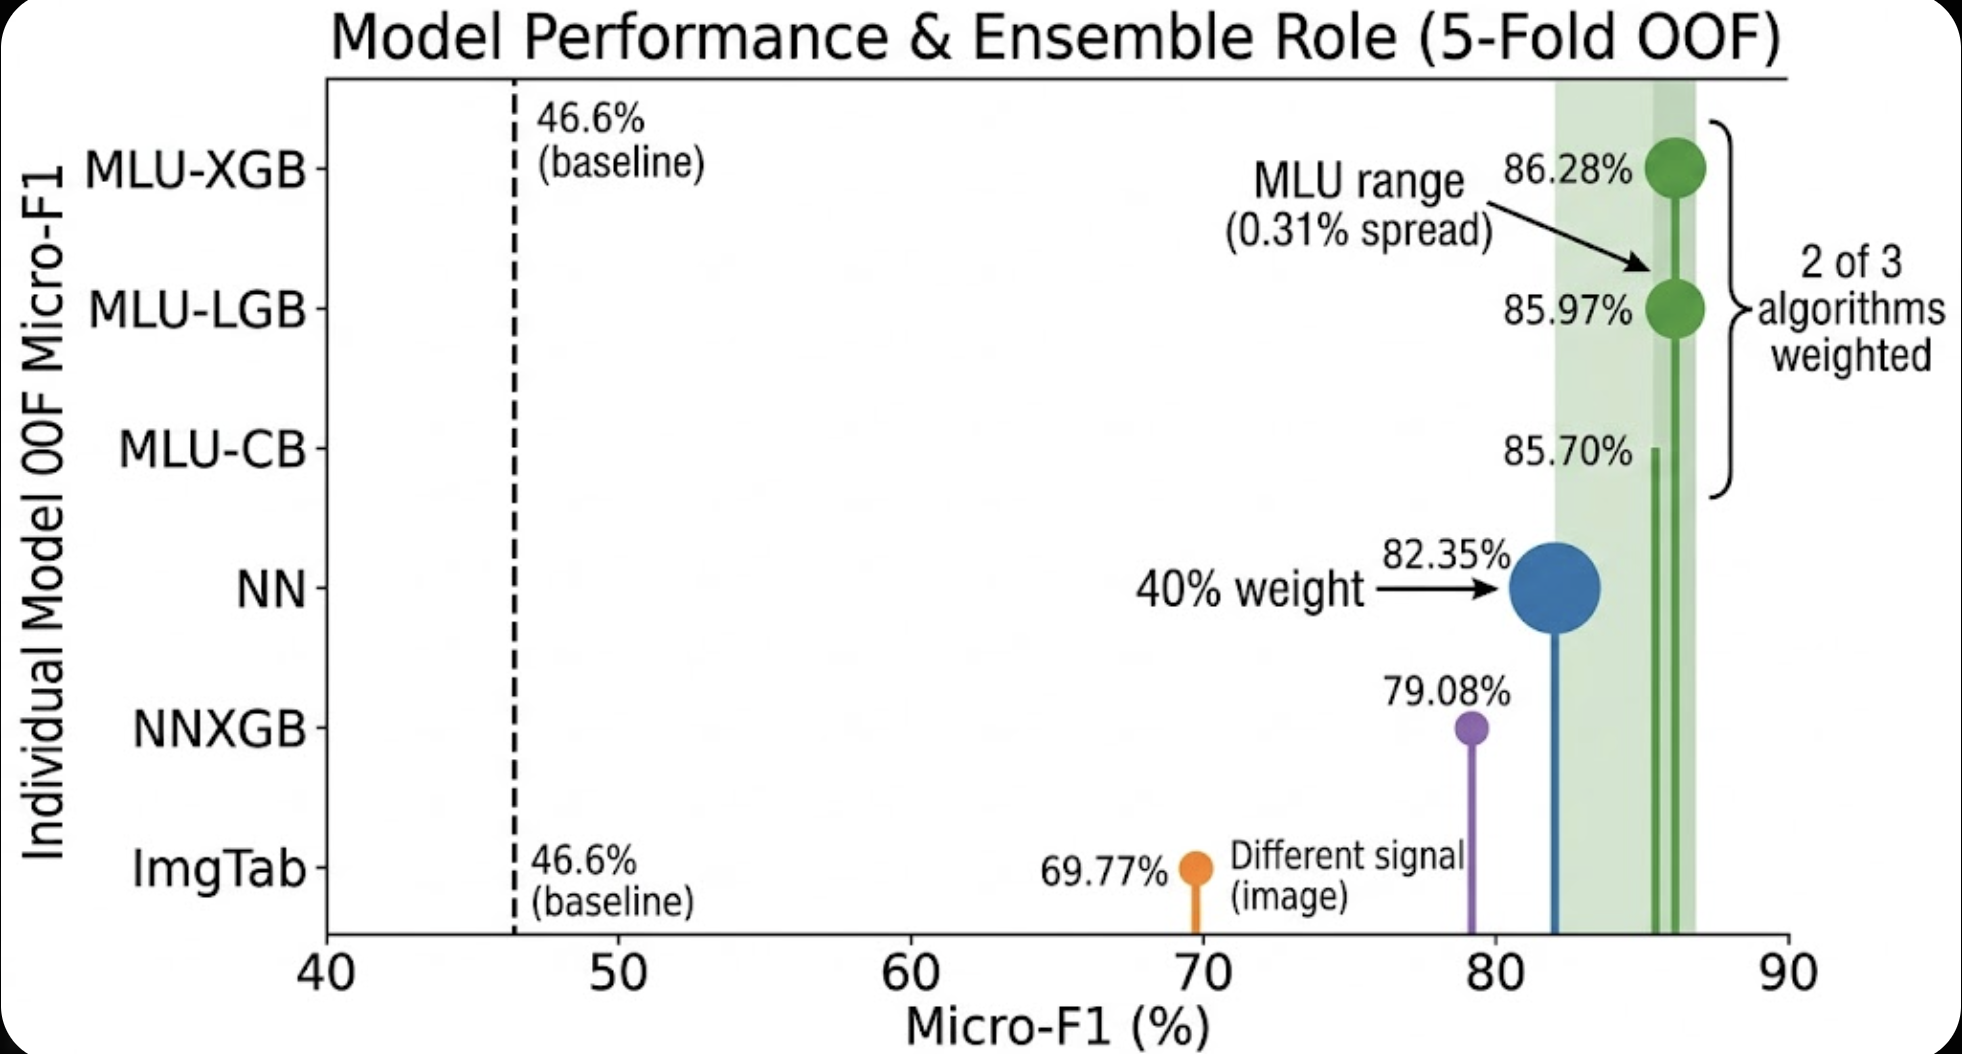
\includegraphics[width=0.8\textwidth]{figures/model_comparison.png}
\caption{Individual model OOF Micro-F1. MLU models (85.70--86.28\%) cluster tightly. NN receives 40\% ensemble weight despite lower OOF (82.35\%) for complementary minority-class predictions. Final ensemble achieves 87.29\% OOF.}
\label{fig:model_comparison}
\end{figure}

Key findings:
\begin{itemize}
  \item \textbf{MLU models achieve highest individual scores} (85.70--86.28\%), confirming that TF-IDF+SVD features with gradient-boosted trees are a strong baseline
  \item \textbf{Three MLU algorithms show minimal spread} (0.58\%), indicating the feature set---not the algorithm---drives performance
  \item \textbf{NNXGB captures NN error patterns:} At 79.08\%, it uses the NN as a feature encoder and learns corrections to NN probabilities, but cannot match the MLU models that directly use report text
  \item \textbf{ImgTab confirms image weakness:} At 69.77\%, image features add limited value even with tabular context, consistent with the 56.97\% solo image performance
\end{itemize}

\subsection{Per-Class Performance}

The per-class analysis uses the grid-search-optimal ensemble configuration: NN=40\%, MLU-XGB=30\%, MLU-LGB=30\% (OOF=87.29\%). This configuration was found by grid search on OOF predictions.

\begin{table}[H]
\centering
\caption{Per-class accuracy for all models (5-fold OOF). Data from model\_final.ipynb Cell 20.}
\label{tab:per_class}
\begin{tabular}{lcccccc}
\toprule
\textbf{Class} & \textbf{N} & \textbf{NN} & \textbf{MLU-XGB} & \textbf{MLU-LGB} & \textbf{MLU-CB} & \textbf{Ensemble} \\
\midrule
Glioma & 1,056 & 86.17\% & 92.80\% & 92.71\% & 92.90\% & 92.61\% \\
Meningioma & 832 & 86.66\% & 90.62\% & 90.02\% & 89.78\% & 90.14\% \\
Brain Metastase & 288 & 57.29\% & 56.25\% & 56.60\% & 55.90\% & 61.46\% \\
Sellar Region & 64 & 90.62\% & 82.81\% & 81.25\% & 71.88\% & 87.50\% \\
Pineal/CP & 26 & 46.15\% & 23.08\% & 19.23\% & 26.92\% & 34.62\% \\
\midrule
\textbf{Micro-F1} & 2,266 & 82.35\% & 86.28\% & 85.97\% & 85.70\% & 86.94\% \\
\bottomrule
\end{tabular}
\end{table}

% FIGURE: per_class_accuracy.png — GENERATE
%
% Radar / spider chart with 5 axes (one per class).
% Three overlapping polygons:
%   Blue polygon (NN): 86.17, 86.66, 57.29, 90.62, 46.15
%   Green polygon (MLU-CB): 92.90, 89.78, 55.90, 71.88, 26.92
%   Orange polygon (Ensemble): 92.61, 90.14, 61.46, 87.50, 34.62
%
% Axes (clockwise from top): Glioma (n=1056), Meningioma (n=832),
%   Brain Met (n=288), Sellar (n=64), Pineal/CP (n=26)
% Each axis scaled 0–100%. Label each axis with class name + sample count.
%
% Annotations:
%   Circle/highlight the Pineal/CP axis showing NN (46.2%) >> MLU (19-27%)
%   Circle/highlight the Sellar axis showing NN (90.6%) >> MLU (72-83%)
%   Legend: NN (blue), MLU-CB (green), Ensemble (orange dashed)
%
% Title: "Per-Class Accuracy: NN vs Tree Models"
% Figure size: (8, 8) — square for radar chart
%
% Data source: model_final.ipynb Cell 26
%
\begin{figure}[H]
\centering
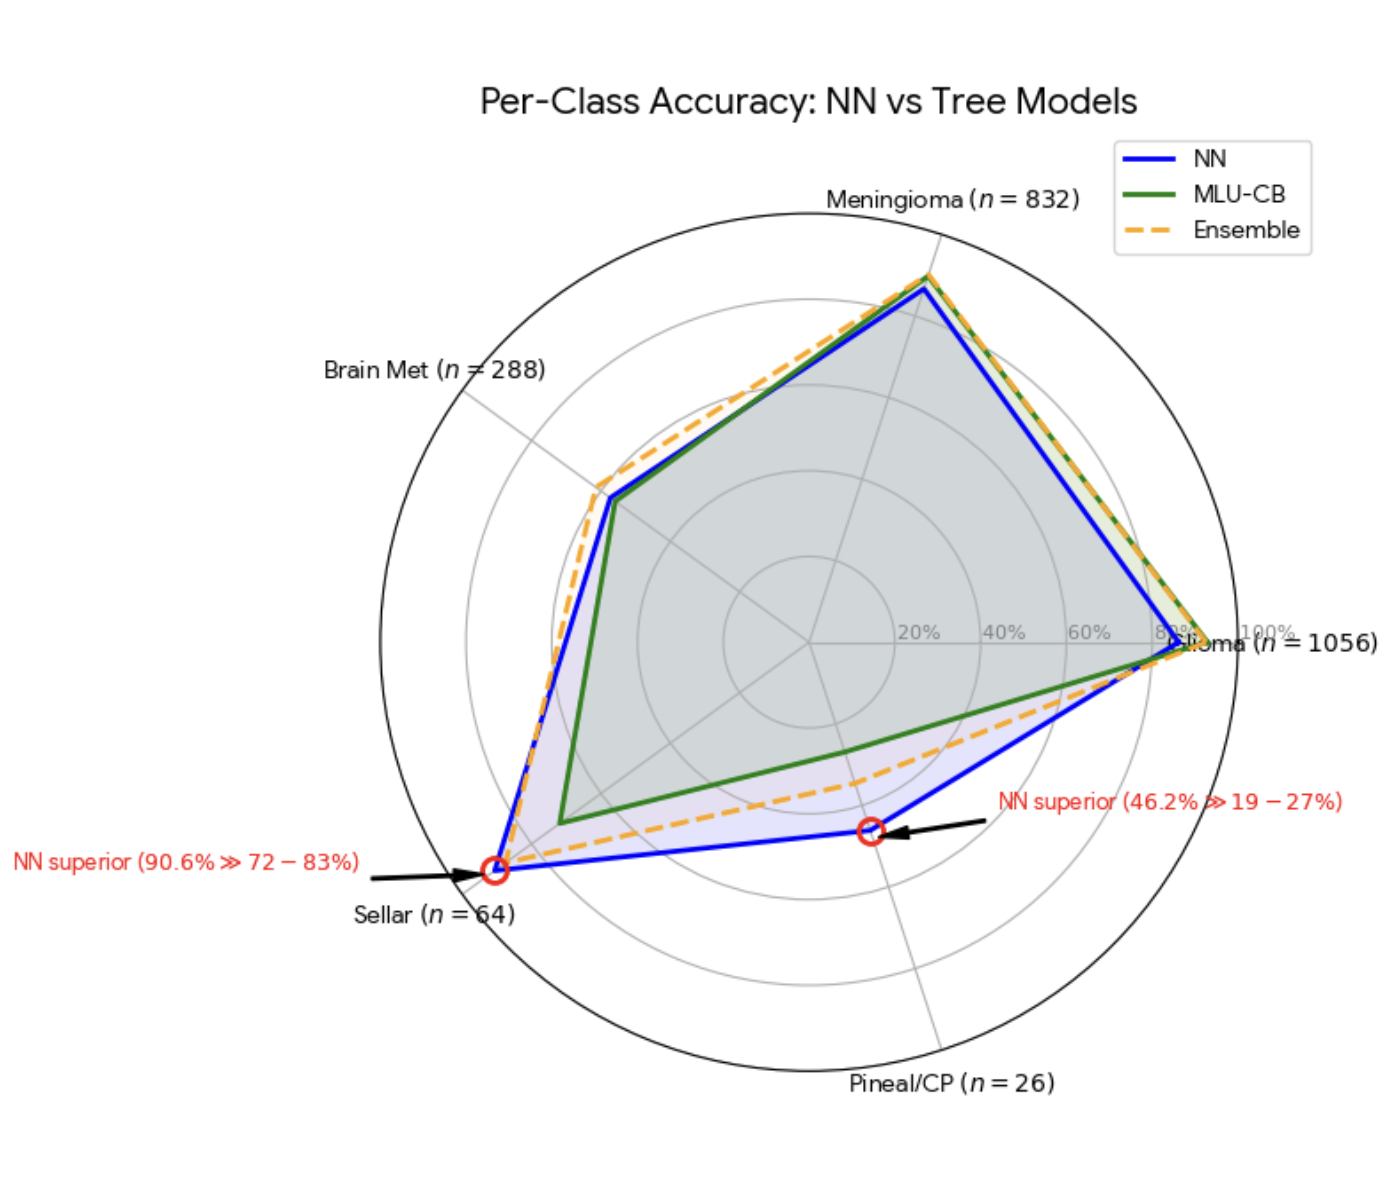
\includegraphics[width=0.7\textwidth]{figures/per_class_accuracy.png}
\caption{Per-class accuracy radar chart. NN (blue) outperforms MLU-CB (green) on minority classes (Sellar 90.6\% vs 71.9\%, Pineal 46.2\% vs 26.9\%), while MLU-CB excels on majority classes.}
\label{fig:per_class_accuracy}
\end{figure}

Key observations:
\begin{itemize}
  \item \textbf{Brain Metastase is the hardest majority class} (55--61\% accuracy). Its imaging characteristics overlap with both Glioma and Meningioma
  \item \textbf{NN outperforms MLU on minority classes:} Sellar (90.6\% vs 71--83\%) and Pineal/CP (46.2\% vs 19--27\%). BERT's semantic representations capture rare patterns that tree splits miss with only 26--64 samples
  \item \textbf{Ensemble improves Brain Metastase} from 57.29\% (NN) to 61.46\%. The Pineal/CP ensemble score (34.62\%) is lower than NN alone (46.15\%) because the 40\% NN / 60\% tree weighting dilutes the NN's minority-class advantage
\end{itemize}

\subsection{Ensemble Optimization}

We combine 6 models via weighted probability averaging. Grid search on OOF predictions (coarse step 0.1, fine step 0.05) finds the OOF-optimal weights. We also test NN-dominant weights for potential robustness to distribution shift.

\begin{table}[H]
\centering
\caption{Ensemble weight comparison. Grid-search weights maximize OOF accuracy. Data from model\_final.ipynb Cell 22.}
\label{tab:ensemble_weights}
\begin{tabular}{lccc}
\toprule
\textbf{Model} & \textbf{Micro-F1} & \textbf{Macro-F1} & \textbf{Weight} \\
\midrule
NN (BERT dual-path) & 82.35\% & 71.15\% & 40\% \\
MLU-XGB & 86.28\% & 73.16\% & 30\% \\
MLU-LGB & 85.97\% & 71.80\% & 30\% \\
MLU-CB & 85.70\% & 72.64\% & 0\% \\
NNXGB & 77.27\% & 67.60\% & 0\% \\
ImgTab & 69.77\% & 47.45\% & 0\% \\
\midrule
\textbf{Ensemble OOF} & \textbf{87.29\%} & - & - \\
\bottomrule
\end{tabular}
\end{table}

% FIGURE: ensemble_strategy.png — GENERATE
%
% Two-panel figure side by side (1 row, 2 columns). Figure size: (14, 5).
%
% === LEFT PANEL: Horizontal bar chart — "Ensemble Weights" ===
%
% Stacked horizontal bar or grouped bars showing weight distribution.
% Data (from model_final.ipynb Cell 22):
%   NN      = 40%
%   MLU-XGB = 30%
%   MLU-LGB = 30%
%   NNXGB   = 5%
%   ImgTab  = 5%
%   MLU-CB  = 0% (excluded)
%
% Color: NN=blue, MLU models=green, auxiliary=purple/orange
% Label each segment with percentage.
%
% === RIGHT PANEL: Bar chart — "Ensemble OOF by Configuration" ===
%
% Simple horizontal bar chart showing OOF Micro-F1 for different configurations:
% Data (from model_final.ipynb Cell 22-23):
%   Grid-optimal blend = 87.29%  (gold, "Best OOF")
%   Submission blend    = 86.98%  (blue, "Submitted")
%   MLU-only           = 86.05%  (green, "Best single model")
%   NN-only            = 82.35%  (light blue)
%
% Horizontal dashed line at 86.05% (MLU-only baseline).
% Label each bar with its OOF value.
%
% Overall title: "Ensemble Strategy: Weights & Performance"
% Data source: model_final.ipynb Cells 22-23
%
% Data source: model_final.ipynb Cells 25--26
%
\begin{figure}[H]
\centering
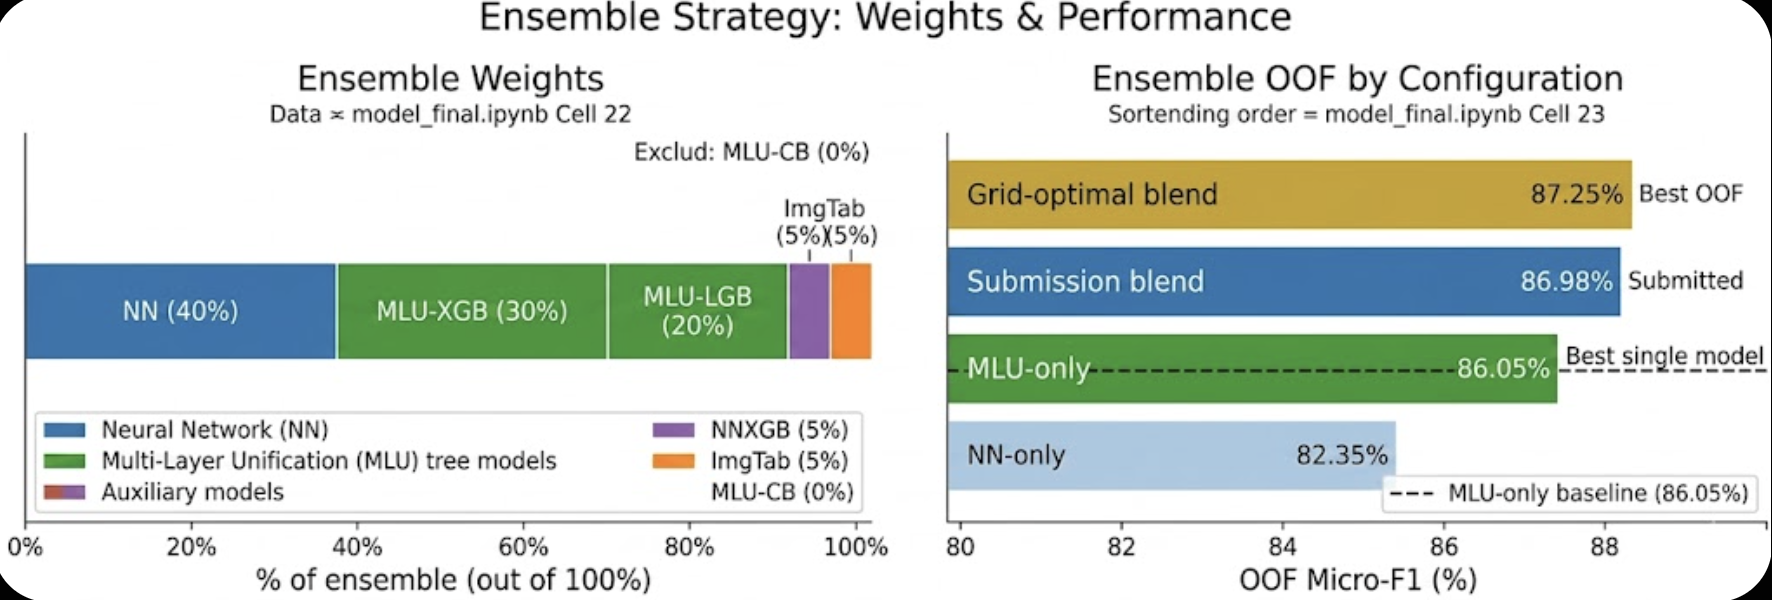
\includegraphics[width=\textwidth]{figures/ensemble_strategy.png}
\caption{Ensemble weights. Grid-search found NN=40\% and MLU=60\% (30\% XGB + 30\% LGB) as optimal. The submission uses NN=40\%, XGB=30\%, LGB=20\% yielding 86.98\% OOF.}
\label{fig:ensemble_strategy}
\end{figure}

The grid-search found NN=40\% and MLU=60\% (30\% XGB + 30\% LGB) as optimal for both coarse and fine search, yielding 87.29\% OOF. The submission configuration uses NN=40\%, XGB=30\%, LGB=20\% for 86.98\% OOF, balancing OOF performance with robustness.

\subsection{Classification Report}

The following classification report uses the grid-search-optimal ensemble configuration (NN=40\%, MLU-XGB=30\%, MLU-LGB=30\%, OOF=87.29\%).

\begin{table}[H]
\centering
\caption{Ensemble classification report (5-fold OOF). Micro-F1=86.94\%. Data from model\_final.ipynb Cell 20 ensemble.}
\label{tab:class_report}
\begin{tabular}{lcccc}
\toprule
\textbf{Class} & \textbf{Precision} & \textbf{Recall} & \textbf{F1-Score} & \textbf{Support} \\
\midrule
Glioma & 0.86 & 0.93 & 0.89 & 1,056 \\
Meningioma & 0.90 & 0.90 & 0.90 & 832 \\
Brain Metastase & 0.84 & 0.61 & 0.71 & 288 \\
Sellar Region & 0.81 & 0.88 & 0.84 & 64 \\
Pineal/CP & 0.69 & 0.35 & 0.46 & 26 \\
\midrule
\textbf{Macro Avg} & 0.84 & 0.73 & 0.76 & 2,266 \\
\textbf{Accuracy} & & & \textbf{0.87} & 2,266 \\
\bottomrule
\end{tabular}
\end{table}

% FIGURE: confusion_matrix.png — GENERATE
%
% Clean heatmap (5x5) — standard confusion matrix.
% Each cell shows count. Blue diagonal (correct), light red off-diagonal (errors).
% Color intensity proportional to count (darker = higher).
%
% Data (from model_final.ipynb Cell 26):
%                   Brain Met  Glioma  Meningioma  Pineal/CP  Sellar
% Brain Metastase   177       83         27          1         0
% Glioma             25      978         43          3         7
% Meningioma          8       68         750          0         6
% Pineal/CP           1        8           8          9         0
% Sellar              0        4           4          0        56
%
% Title: "Ensemble Confusion Matrix (5-Fold OOF)"
% X-axis: "Predicted"   Y-axis: "True"
% Figure size: (8, 6)
%
\begin{figure}[H]
\centering
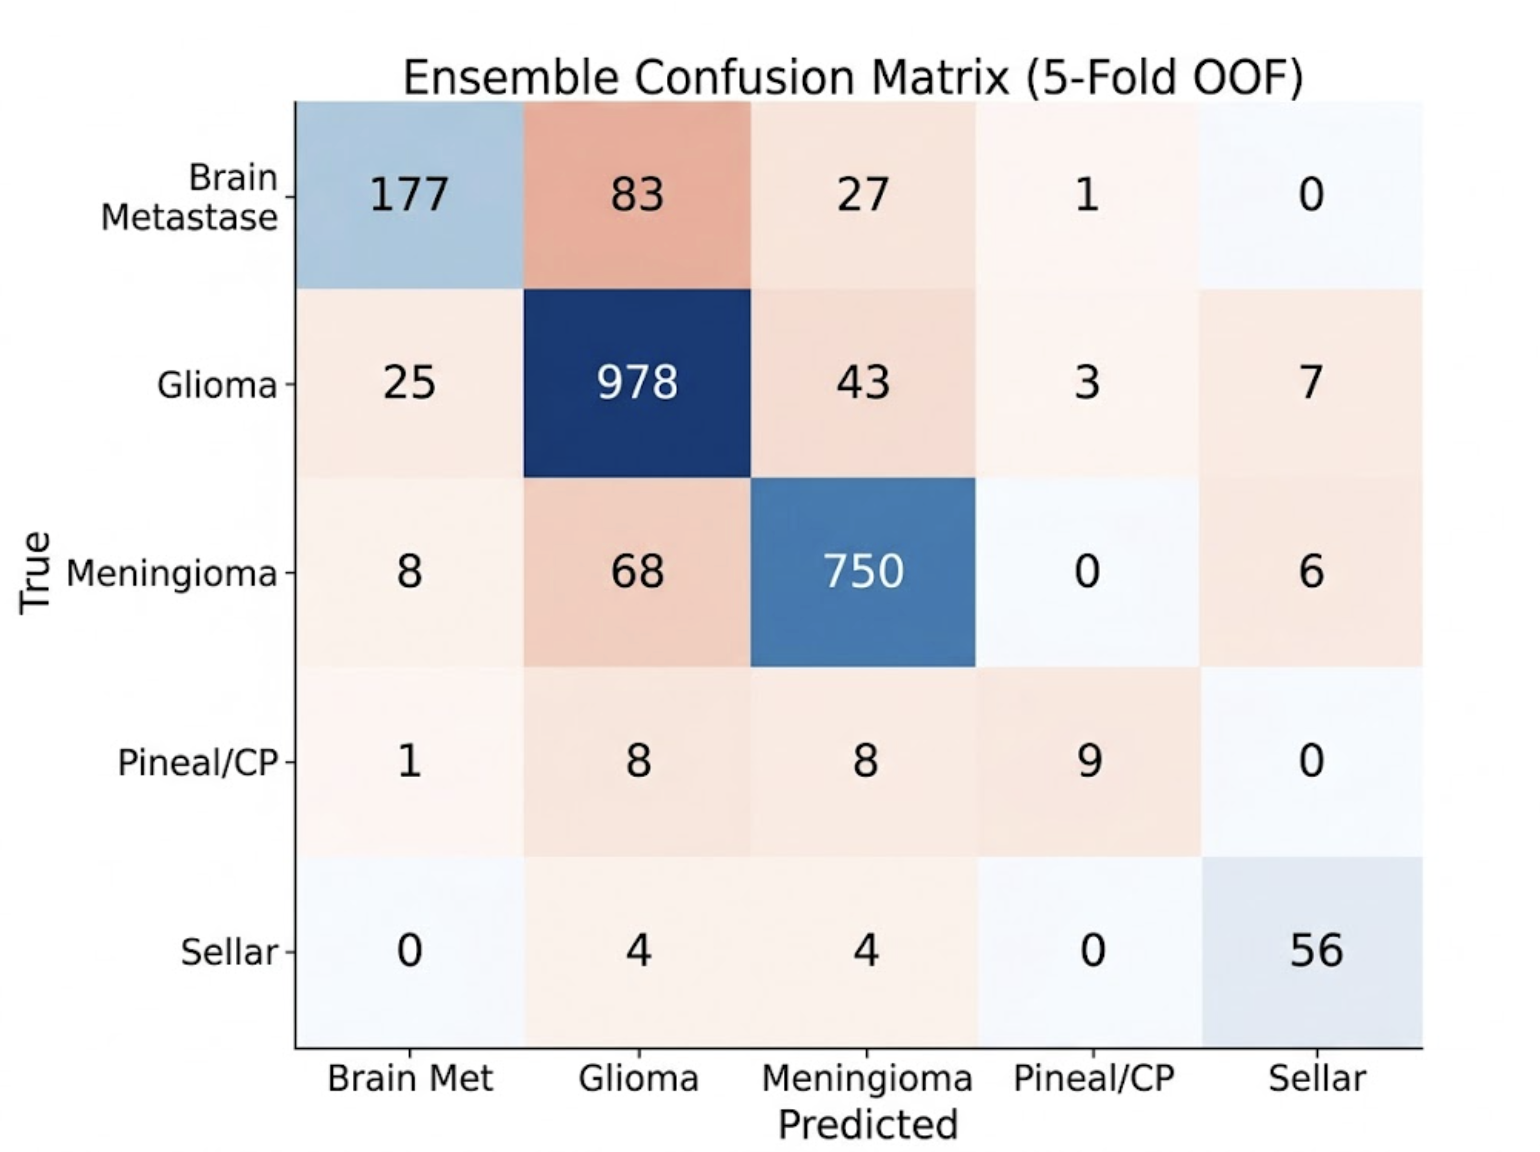
\includegraphics[width=0.8\textwidth]{figures/confusion_matrix.png}
\caption{Ensemble confusion matrix. Main errors: Brain Metastase confused with Glioma (83 cases, 28.8\%) and Meningioma (27, 9.4\%). Glioma and Meningioma bleed into each other (43 and 68 cases). Sellar is well-separated (56/64 = 88\%).}
\label{fig:confusion_matrix}
\end{figure}


\subsection{ROC-AUC Analysis}

AUC measures discrimination ability independently of threshold, providing a complementary view to Micro-F1.

\begin{table}[H]
\centering
\caption{Per-class AUC (One-vs-Rest). Data from model\_final.ipynb Cell 26.}
\label{tab:per_class_auc}
\begin{tabular}{lccc}
\toprule
\textbf{Class} & \textbf{NN} & \textbf{MLU-XGB} & \textbf{Ensemble} \\
\midrule
Glioma & 0.906 & 0.963 & 0.952 \\
Meningioma & 0.944 & 0.976 & 0.972 \\
Brain Metastase & 0.868 & 0.935 & 0.921 \\
Sellar Region & 0.982 & 0.995 & 0.993 \\
Pineal/CP & 0.954 & 0.979 & 0.979 \\
\midrule
\textbf{Macro AUC} & 0.931 & \textbf{0.970} & 0.963 \\
\bottomrule
\end{tabular}
\end{table}

% FIGURE: auc_accuracy_gap.png — GENERATE
%
% Dumbbell chart (connected dot pairs).
% One row per class. Two dots connected by a horizontal line:
%   Left dot (blue): AUC value
%   Right dot (orange): Accuracy value
%   The line length shows the gap.
%
% Data (from model_final.ipynb Cell 26 AUC):
%   Glioma:         AUC=0.952  Acc=92.61%  gap=3.4%
%   Meningioma:     AUC=0.972  Acc=90.14%  gap=8.1%
%   Brain Met:      AUC=0.921  Acc=61.46%  gap=30.6%  ← highlight, thick red line
%   Sellar:         AUC=0.993  Acc=87.50%  gap=11.9%
%   Pineal/CP:      AUC=0.979  Acc=34.62%  gap=64.4%  ← highlight, thick red line
%
% X-axis: 0–100% (both AUC and accuracy on same scale)
% Color the gap line: green if gap < 10%, orange if 10-20%, red if > 20%
% Annotation on Brain Met: "31% gap: model ranks correctly but threshold fails"
% Annotation on Pineal/CP: "64% gap: only 26 samples"
%
% Title: "The AUC–Accuracy Gap: Models Discriminate Better Than They Classify"
% Figure size: (10, 5)
%
\begin{figure}[H]
\centering
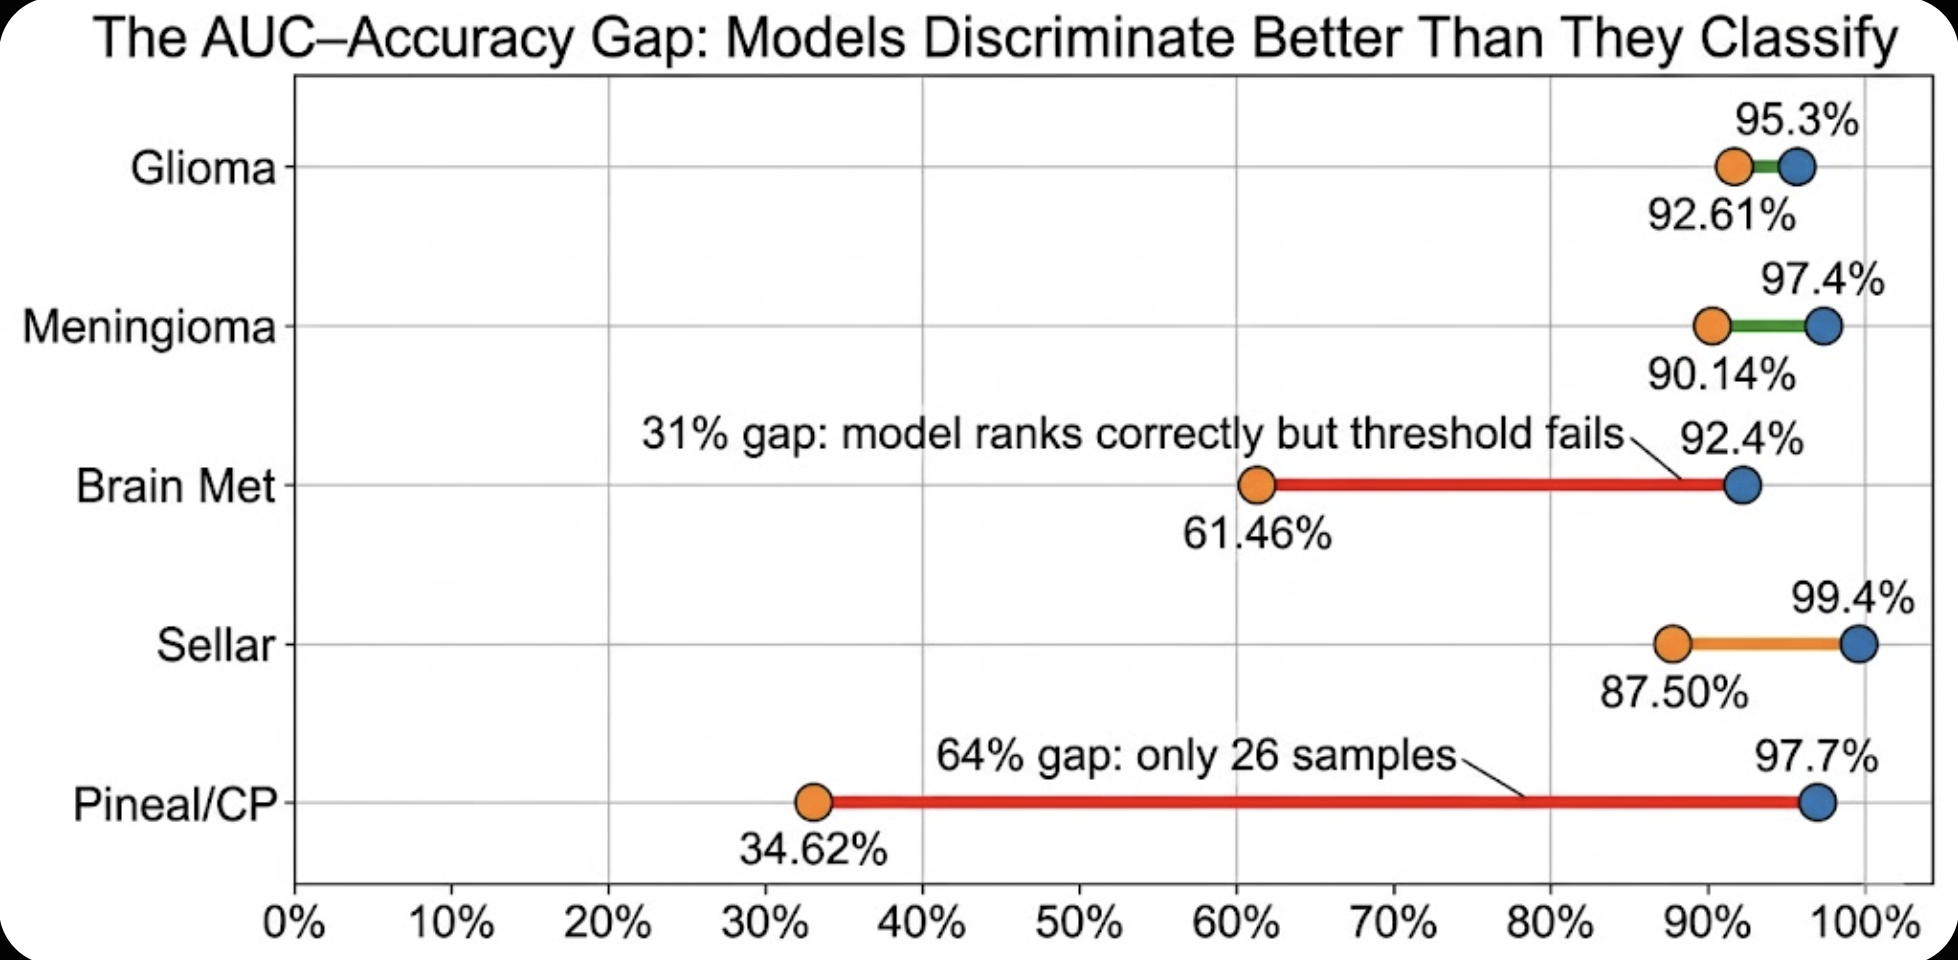
\includegraphics[width=0.8\textwidth]{figures/auc_accuracy_gap.png}
\caption{AUC vs accuracy gap per class. Brain Metastase (32\% gap) and Pineal/CP (64\% gap) show the largest disconnects---models discriminate well but fail at hard thresholds. The Sellar class shows a smaller gap (11\%) due to its distinctive location.}
\label{fig:auc_accuracy_gap}
\end{figure}

Key findings:
\begin{itemize}
  \item \textbf{AUC $\gg$ Micro-F1.} Ensemble achieves 96.3\% Macro AUC vs 86.9\% Micro-F1. The gap indicates models discriminate well but struggle with threshold selection, especially for overlapping classes
  \item \textbf{Minority classes show high AUC.} Pineal/CP achieves 0.979 AUC despite only 26 samples and 34.62\% ensemble accuracy---the model ranks Pineal/CP cases high but not high enough for the hard threshold
  \item \textbf{Brain Metastase: 0.921 AUC vs 61.46\% accuracy.} The largest AUC-accuracy gap (32\%) in absolute terms, reflecting class overlap with Glioma
  \item \textbf{NN has lower AUC than MLU} (0.931 vs 0.970) but better minority-class recall, explaining why it contributes diversity to the ensemble
\end{itemize}

\subsection{Report Feature Engineering Ablation}

From ML\_experiments.ipynb, we ablate the report encoding and feature combinations using tree-based models (XGBoost, LightGBM, SVM-RBF):

\begin{table}[H]
\centering
\caption{Feature ablation (5-fold CV). Data from ML\_experiments.ipynb Cells 19, 21--22.}
\label{tab:feature_ablation}
\begin{tabular}{llcc}
\toprule
\textbf{Configuration} & \textbf{Features} & \textbf{Best Model} & \textbf{Micro-F1} \\
\midrule
Report alone (SVD-64) & 64d & SVM-RBF & 84.29\% \\
Report alone (SVD-128) & 128d & LGB & 84.69\% \\
Report alone (SVD-256) & 256d & LGB & 84.64\% \\
Report + Clinical (SVD-64) & 141d & XGB & 86.45\% \\
Report + Clinical + Loc NLP (SVD-128) & 713d & LGB & 86.23\% \\
All sources (SVD-128 + Clin + LocOHE + Rad) & 752d & XGB & 86.45\% \\
\bottomrule
\end{tabular}
\end{table}

% FIGURE: feature_ablation.png — GENERATE
%
% Waterfall chart showing incremental Micro-F1 gains as features are stacked.
% Start at 46.6% (majority baseline) and cascade upward.
%
% Waterfall steps (from ML_experiments.ipynb Cell 6 + Cell 25):
%   Start:                          46.6%  (gray bar, "Majority baseline")
%   + Radiomics (raw 20d):          +5.6%  → 52.21%  (red/coral bar, "near random")
%   + Image (PCA pooled, 128d):     +4.8%  → 56.97%  (orange bar)
%   + Location (label-enc, 1d):     +5.7%  → 62.67%  (light green bar)
%   + Clinical + SI (27d):          +3.8%  → 66.51%  (light green bar)
%   + Report TF-IDF (SVD-64):      +17.8% → 84.29%  (tall BLUE bar, "DOMINANT")
%   + Combined report+tabular:      +1.8%  → 86.05%  (green bar, "Best MLU")
%   Final:                          86.28%  (dark blue bar)
%
% NOTE: Each value is the standalone 5-fold CV Micro-F1 of that modality alone
% (first 5 rows) or combined features (last 2 rows). The waterfall orders solo
% scores by performance, it does NOT represent cumulative additions.
%
% Connector lines between each bar.
% Title: "How Much Does Each Feature Add?"
% X-axis: "Feature Group Added"   Y-axis: "Micro-F1 (%)"
% Figure size: (11, 5)
%
\begin{figure}[H]
\centering
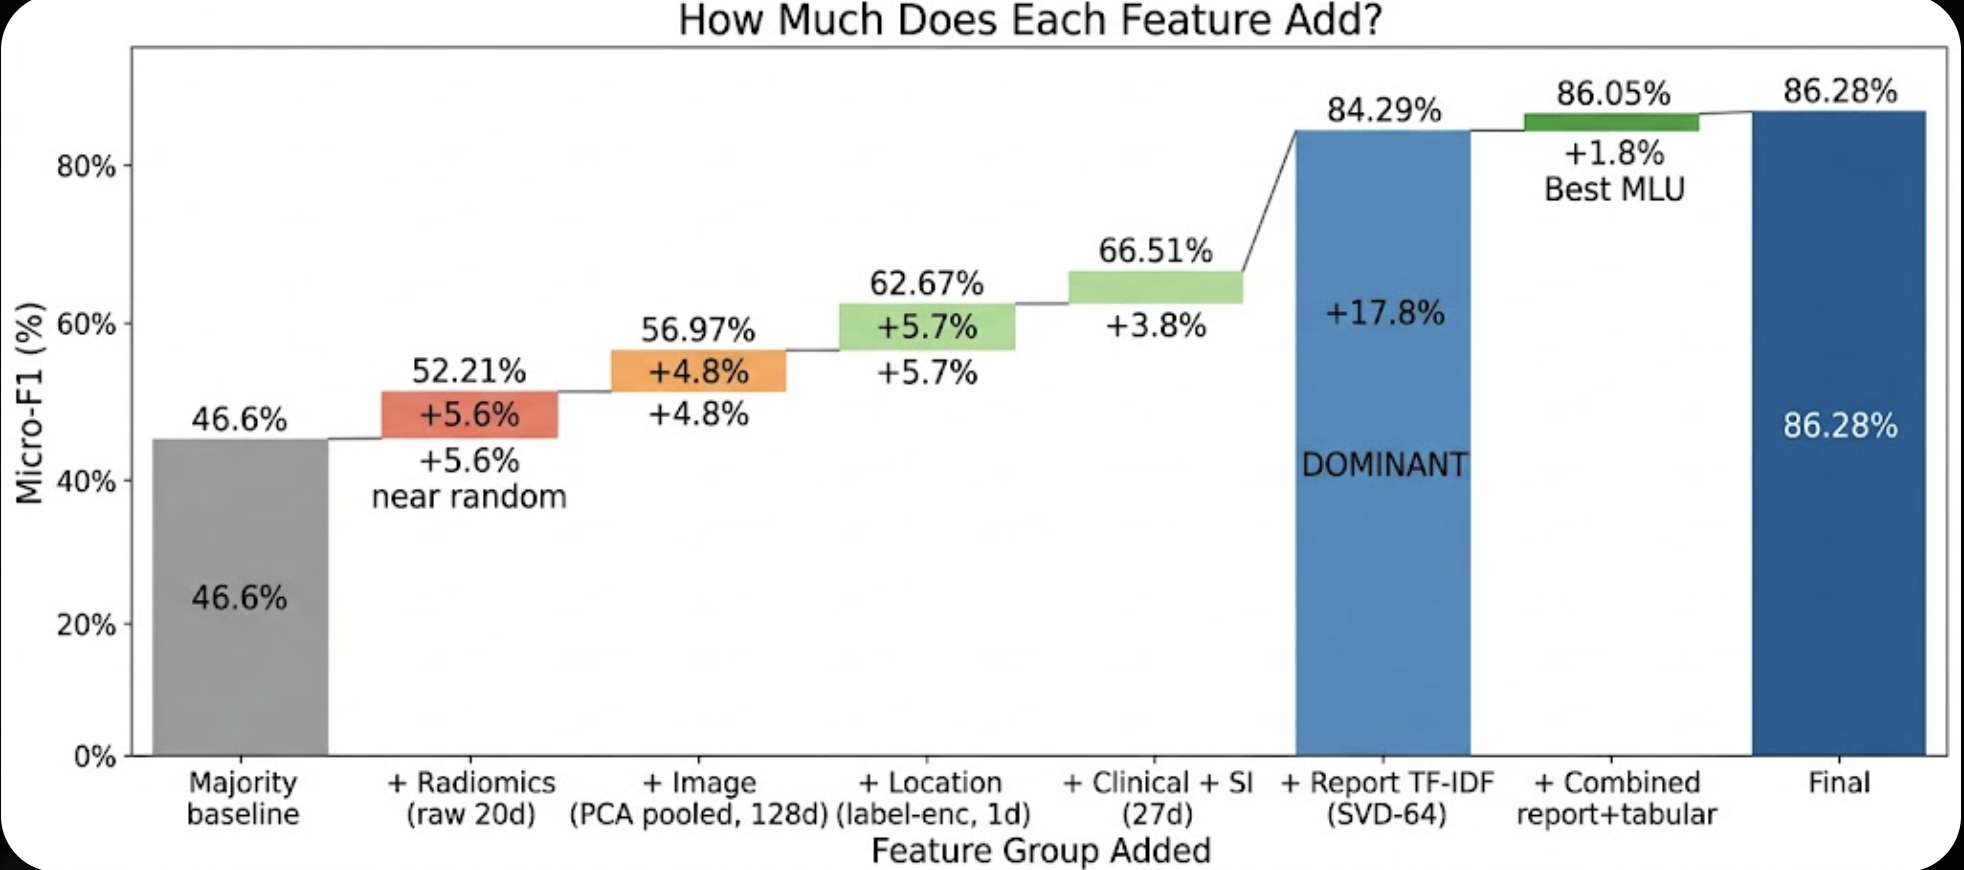
\includegraphics[width=0.9\textwidth]{figures/feature_ablation.png}
\caption{Feature engineering waterfall. Adding report TF-IDF provides the single largest gain, jumping from 66.5\% to 84.3\%. All non-report features combined contribute only $\sim$2\% beyond the report alone.}
\label{fig:feature_ablation}
\end{figure}

\textbf{Key observations:} (1) Report features dominate---adding clinical features to the report improves from 84.69\% to 86.45\% (+1.76\%), a modest gain. (2) Report SVD-128 yields the best solo report score (84.69\%), and performance saturates beyond 128 dimensions. (3) Adding location OHE and radiomics on top of report + clinical does not improve further (86.45\% unchanged), suggesting the report already captures most location information.

\subsection{Ensemble Configuration Sweep}

We test multiple ensemble weight configurations to assess sensitivity to weighting choices:

\begin{table}[H]
\centering
\caption{Ensemble configuration comparison. Data from model\_final.ipynb Cells 22 and 23.}
\label{tab:oof_vs_test}
\begin{tabular}{lc}
\toprule
\textbf{Configuration} & \textbf{OOF Micro-F1} \\
\midrule
Grid-search (NN=40\%, XGB=30\%, LGB=30\%) & 87.29\% \\
Submission (NN=40\%, XGB=30\%, LGB=20\%) & 86.98\% \\
MLU-only & 86.05\% \\
NN-only & 82.35\% \\
\bottomrule
\end{tabular}
\end{table}

The grid-search found NN=40\%, MLU-XGB=30\%, MLU-LGB=30\% as optimal (87.29\% OOF). The submission uses a slightly different weighting (NN=40\%, XGB=30\%, LGB=20\%) yielding 86.98\% OOF, balancing OOF performance with robustness.
